\documentclass{beamer}
\usepackage{graphicx}
\usetheme{metropolis}

\title[BB84]{BB84}
\subtitle{A Quantum Key Distribution Protocol}
\author[Team 37]{Lakshika, Shreya}
\date{July 2020}


\begin{document}

\begin{frame}
	\titlepage
\end{frame}

\begin{frame}
	\frametitle{Overview}
	 Simulation of BB84 Protocol
\end{frame}


\begin{frame}[standout]
    \begin{columns}
        \column{0.38\linewidth}
            \centering
            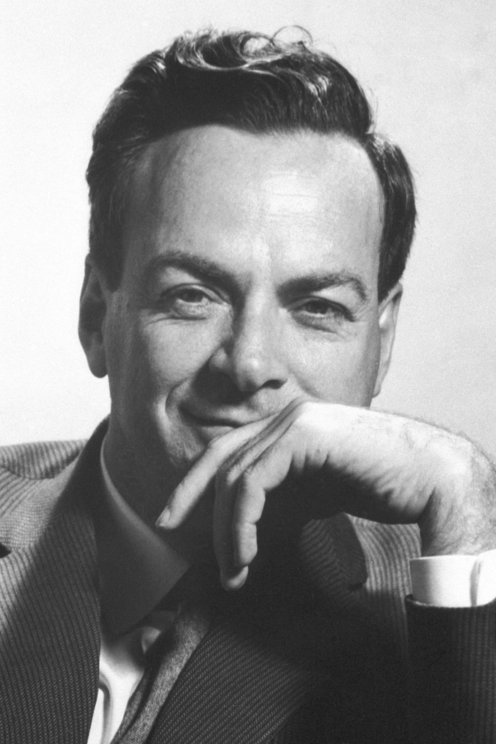
\includegraphics{feynman.jpg}
        \column{0.58\linewidth}
            \emph{Nature isn’t classical, dammit, and if you want to make a simulation of nature, you’d better make it quantum mechanical...}
        \begin{flushright}
            - Richard Feynman
        \end{flushright}
    \end{columns}
\end{frame}


\begin{frame}{Technology Stack}
	\begin{itemize}
		\item Qiskit - An SDK for Quantum Computing
		\item IBM Q - IBM Quantum Experience to access IBM's quantum computers via the cloud
	\end{itemize}
\end{frame}


\begin{frame}{Quantum Key Distribution}
    \begin{itemize}[<+->] 
        \item Cryptographic protocols are used for secure communication
        \item The parties involved require a common key for these protcols
        
        \item BB84 is the first Quantum Key Distribution protocol
    \end{itemize}
\end{frame}

\begin{frame}{Description}
    \begin{itemize}
        \item A QKD protocol that provides a way to share an unconditionally secure key in the presence of an eavesdropper.\\
        \item We require two different communication channels : \\
            \textbf{Quantum Communication Channel} \\
            \begin{itemize}
                \item Transfer of quantum information
                \item Adversary has full access i.e. can intercept, alter, store and resend
            \end{itemize}
            \textbf{Classical Authenticated Channel} \\
            \begin{itemize}
                \item Unaltered message guaranteed
                \item Adversary can read all the messages
            \end{itemize}
    \end{itemize}
\end{frame}

\begin{frame}{BB84 Protocol}
    \begin{itemize}[<+->]
        \item \textbf{Pseudo key production} -  using QCC and CAC
        \item \textbf{Information Reconciliation} - exchange error-correcting information to improvise receiver's noisy version of key
        \item \textbf{Privacy Amplification} -  production of final secure key 
    \end{itemize}
\end{frame}


\begin{frame}{Timeline}
    \begin{tabular}{ll}
            23rd - 24th June & Domain selection and resources collection\\
            25th - 30th June & Audited a course on Quantum Computing\\
            1st - 7th July & Read \emph{Dancing with Qubits}, chose Cryptography\\
            8th - 14th July & Audited course on Quantum Cryptography, chose BB84\\
            15th - 16th July & Read more notes and collected resources for BB84\\
            17th - 18th July & Implemented the 1st stage of the Protocol\\
            19th - 22nd July & Looked upon research papers\\
            23rd - 26th July & Complete the code\\
            27th - 31st July & Test and debug the code\\
     \end{tabular}
\end{frame}

\begin{frame}{Difficulties faced}
	\begin{itemize}
		\item Getting started with Quantum Computing
        \item In choosing a sub-domain
        \item Unsure about the language and tools to use
	\end{itemize}
\end{frame}
		
\end{document}
